\documentclass[a4paper,12pt]{report}
\usepackage{cmap} % Поиск PDF
\usepackage[T2A]{fontenc}  % Кодировка
\usepackage[utf8]{inputenc}  % Кодировка исходного текста 
\usepackage[english,russian]{babel}  % Кодировка исходного текста 
\usepackage{fontspec}
\usepackage{xcolor}
\usepackage{hyperref}
\definecolor{linkcolor}{HTML}{2d7ac7} % цвет ссылок
\definecolor{urlcolor}{HTML}{2d7ac7} % цвет гиперссылок
\usepackage{graphicx}
\graphicspath{ {./images/} }
\setlength{\parskip}{0.3em}
\newcommand{\contractAddress}{0x37d29cb7d543300063a50d85389d409c01da7945}

\hypersetup{pdfstartview=FitH,  linkcolor=linkcolor,urlcolor=urlcolor, colorlinks=true}

\setmainfont{Ubuntu}
\providecommand{\versionnumber}{2.0}

% Title Page
\title{
\includegraphics[width=14cm]{logo}\\[2cm]Инфраструктура Portal Energy \\\normalsize v\versionnumber}
\author{Иванцов М. Мовчан П. Прусов М. Бутаков С. Патрикеев Б.}

\date{\today}


\begin{document}%
\maketitle
\tableofcontents
\clearpage


\chapter{Вступление}

Portal Energy была основана на слиянии технологий в сфере электроники, IT и Big data. Начиная с 2016 года, работаем над созданием недорогих и универсальных зарядных устройств для электромобилей. 

Тема электротранспорта позволила нам познакомиться и сформироваться в команду, однако, она не является единственной зоной нашего интереса. Со временем, по мере реализации всех поставленных целей, и достижению необходимых финансовых показателей, мы будем работать в сфере возобновляемой энергии, в социальной сфере, в сфере образования, в сфере интернета, и других. У общества много запросов, а у нас есть идеи, как эти запросы удовлетворить. 

\textbf{todo: Тут надо бы вставить наши лица и кратко написать о каждом}

Для превращения слов в конкретный результат, нам нужен эффективный инструмент. На наш взгляд эффективная система, работающая в рамках социума, немыслима без прямого участия представителей этого социума. Ведь именно люди являются носителями знаний о характере и нюансах наиболее актуальных проблем, и они же будут конечными потребителями результатов работы системы. Поэтому мы строим компанию, которая ориентирована, чтобы приносить пользу обществу и вовлекать людей в его развитие. Построить такую компанию и сделать её успешной - наша главная задача. 

В первую очередь, мы формируем сообщество заинтересованных людей, для которого Portal Energy -  инструмент развития электротранспорта.

Точкой старта развитие электротранспорта мы выбрали потому как в нашей стране эта тема находится на этапе зарождения, мы сами являемся её энтузиастами, и в долгосрочной перспективе здесь можно построить отличный фундамент для последующих проектов. 

Данный документ раскрывает наше видение развития электротранспорта в РФ, наши планы и их описание.

Ниже в тексте мы будем использоваться различные технические термины. Их краткое разъяснение дано в глоссарии. Если они вам знакомы, можете сразу переходить к разделу \ref{chapter3}.


\chapter{Глоссарий}

\section{Смарт-контракт}
Смарт-контракты похожи на классические контракты, за исключением того, что третьей стороной является множество людей, которые проверяют контракт на его исполнение и результат этого выполнения у всех участников должен совпадать, только тогда он будет считаться верным. В контракте мы можем прописать любые условия, которые надо выполнить. Из-за того что его выполняют множество участников, то мы не можем себе позволить исполнять очень сложные контракты, т.к. они будут требовать больших вычислительных мощностей. За вычисление берется комиссия в валюте ether(в сети Ethereum). После выполнения контракта сохраняется его состояние в блокчейне,
и удалить эту информацию невозможно.

\section{Блокчейн}
Выстроенная по определённым правилам непрерывная последовательная цепочка блоков, содержащих информацию. Простыми словами это цепочка блоков, каждый из которых обладает меткой времени, ссылкой на предыдущий блок и хранится на разных компьютерах.

\section{Криптовалюта}
Зашифрованный не регулируемый цифровой актив, использующийся в качестве аналога валюты в обменных операциях. Криптовалюта не имеет физической формы, она существует только в электронной сети в виде данных. Единицей такой валюты является «coin» (в переводе на русский –«монета»). При этом монета защищена от подделки, так как монета представляет собой зашифрованную информацию, скопировать которую невозможно.

\section{Ethereum}
Платформа для создания децентрализованных онлайн-сервисов на базе блокчейна (децентрализованных приложений), работающих на базе умных контрактов. Реализована как единая децентрализованная виртуальная машина.

\section{Ether}
Обменная единица Ethereum называются эфиром (англ. ether). Эта единица может делится на дробные части. 1/1000 — finney, 1/106 — szabo, 1/1018 — wei. Этой единицей может владеть как обычный кошелек, так и смарт-контракт. Такими же свойствами обладает и токен POE.

\section{Токен}
Единица учёта, не являющаяся криптовалютой, предназначенная для представления цифрового баланса в некотором активе, иными словами выполняющая функцию «заменителя ценных бумаг» в цифровом мире. Токены представляют собой запись в регистре, распределенную в блокчейн-цепочке.

\section{Токен ERC20}
ERC (Ethereum Request for Comments) — это официальный протокол для внесения предложений по улучшению сети Ethereum; 20 – уникальный идентификационный номер предложения. Технические спецификации для токенов, выпускаемых на блокчейне Ethereum, были опубликованы в 2015 году. Токены, отвечающие этим спецификациям, известны как токены стандарта ERC-20 и фактически являются смарт-контрактами на блокчейне Ethereum. Стандарт ERC-20 определяет набор правил, которые должны быть
соблюдены для того, чтобы токен был принят и имел возможность взаимодействовать с другими токенами в сети. Сами токены представляют собой блокчейн-активы, которые могут иметь ценность, а также могут быть отправлены и получены как любая другая криптовалюта. 

Отличие токенов ERC-20 от других известных криптовалют, напри-
мер, биткоина или Litecoin, в том, что они привязаны к сети Ethereum, используют принятый внутри этой сети формат адресов и отправляются при помощи Ethereum-транзакций. Соответственно, транзакции с участием токенов ERC-20 можно прослеживать в обозревателе блоков.


\href{https://etherscan.io/address/\contractAddress}{Здесь} можно отследить движение всех наших токенов.


\section{Etherscan}
Сервис для просмотра статистики сети Ethereum. С помощью него Вы можете просматривать. Основная функция Etherscan — отслеживание проводимых переводов. С помощью него Вы можете проверить статус вашей операции, проверить адреса и получить прочую информацию  \href{https://etherscan.io/}{https://etherscan.io/}.


\section{DAO/ДАО}
\label{dao}

ДАО (Децентрализованная Автономная Организация) — это новая парадигма экономического сотрудничества. Как следует из названия, ДАО принципиально отличается от обычной компании децентрализованной структурой и автономностью.

Децентрализованность означает горизонтальное строение компании. У ДАО нет единоличного владельца или совета директоров, каждый участник организации — полноправный совладелец и обладает равными полномочиями и неограниченным доступом к информации.

Инструментом, позволяющим обеспечить подобную структуру, является блокчейн. Блокчейн в данном случае является электронным реестром компании, который поддерживается и удостоверяется всеми участниками сети.

Автономность обеспечивается независимостью от традиционных финансовых и политических институтов, и важную роль в этом играет замена обычных денег криптовалютой. При этом криптовалюта, как и любая блокчейн-система, сама по себе может быть классифицирована как ДАО, так как имеет децентрализованную структуру, а большинство процессов в ней автономны.

Более того, система ДАО делает ненужной корпоративную юриспруденцию, так как все взаимодействия внутри и между ДАО осуществляются с помощью умных контрактов — программной инфраструктуры, которая задает приемлемые для абсолютного большинства участников правила игры и обеспечивает простоту в заключении контрактов, проведении транзакций и т. д. В завершенной форме ДАО не только абсолютно автономна, но и максимально или полностью автоматизирована.

Если всякая традиционная компания опирается на сеть легальных, финансовых и политических инструментов, предоставляемых государственными институтами, то ДАО использует автономную и горизонтальную цифровую структуру. Использование ДАО в рамках классических коммерческих структур, например, для частичной автоматизации или оптимизации операционных процессов, будь то бухгалтерское производство или правовое сопровождение деятельности компании.

По сравнению с традиционными компаниями, ДАО обеспечивают своим участникам больший контроль над собственными вложениями и общим курсом компании. 

Источник: \href{https://forklog.com/chto-takoe-detsentralizovannye-avtonomnye-organizatsii-i-zachem-oni-nuzhny/}{forklog.com}

\chapter{Электромобили как технология}
\label{chapter3}
Электромобили являются неизбежным будущим автомобильной индустрии. 

Почему это так? 

В первую очередь, электродвигатель гораздо более эффективен, в сравнении с двигателем внутреннего сгорания (далее ДВС) (КПД электродвигателя 95-98\% против 38\% у ДВС). Что уже само по себе выливается в значительную экономию средств (заряжать электромобиль может быть до 6 раз дешевле, чем обычный автомобиль, из расчета на 100 км). Плюс, электропривод экологичен, что для жителей мегаполисов крайне важно. Да и в целом, вопрос экологии становится всё более и более актуальным. 

Мы сделали небольшой обзор масштаба проблемы экологии в крупных городах, насколько грязным воздухом мы дышим, какие это имеет последствия и что нужно делать, чтобы ситуацию исправлять. Чтобы не утяжелять основной документ, здесь мы приводим ссылку на текст. Время чтения - 15 минут (\href{https://docs.google.com/document/d/1Xvn2jIdGmjOemTvSG5J-kHtrBBC3f-odBOGnE6IfGFw}{ссылка})

Кроме того, электромобили значительно манёвреннее и безопаснее обычных автомобилей, в связи с конструктивными отличиями. И, наконец, потенциал электромобиля только начинает раскрываться, в то время, когда потенциал авто с ДВС уже достиг своего предела. 

Однако возникает логичный вопрос - если электромобили лучше по большинству показателей, в разы дешевле в эксплуатации и зарядке, экологичны - почему тогда они массово не распространены в нашей стране? 

Тем самым мы пришли ко второму нашему вопросу.



\chapter{Почему нет массового развития инфраструктуры в России?}
Вопрос действительно хороший. Чтобы вразумительно на него ответить, давайте посмотрим на страны, где электротранспорт уже распространён широко. 

\section{Электромобили в мире}
Лучше всего дела с электромобилями обстоят в Китае. В поднебесной за 2019 год было зарегистрировано более 1.2 млн новых автомобилей, а всего их 3.8 млн. Таже на начало 2019 года в Китае официально зарегистрировано более 1 млн зарядных станций.

На втором месте идут США. Там за 2019 год официально прибавилось 330 тыс. электромобилей. Всего в штатах их более 1.5 млн. штук, при этом зарядных станций там на 2019 год было более 200 тыс. штук.

В Европе, на конец 2019 года, количество электромобилей приблизилось к 2 млн штук, при проданных за год 550 тыс. штук и увеличении продаж в 1.5 раза в начале 2020 года.
Более того, дальнейшее будущее электротранспорта в развитых странах поистине безоблачно. 

Взгляните на графики роста выпуска электромобилей. Эти показатели говорят сами за себя. Стоит отметить, что в эту статистику входят не только абсолютные электромобили, но и подзаряжаемые гибриды (plug-in hybrids), т.к. подавляющее большинство из них имеют достаточно ёмкие батареи и полноценно используют зарядную инфраструктуру.
После 2023 года доля таких гибридов сокращается в пользу электромобилей.

Цифрами в перевёрнутых треугольниках обозначены некоторые из событий, ускоряющих смену автопарка на планете с ДВС на электро, либо являющихся важными контрольными точками этих изменений.

\vspace*{1cm}
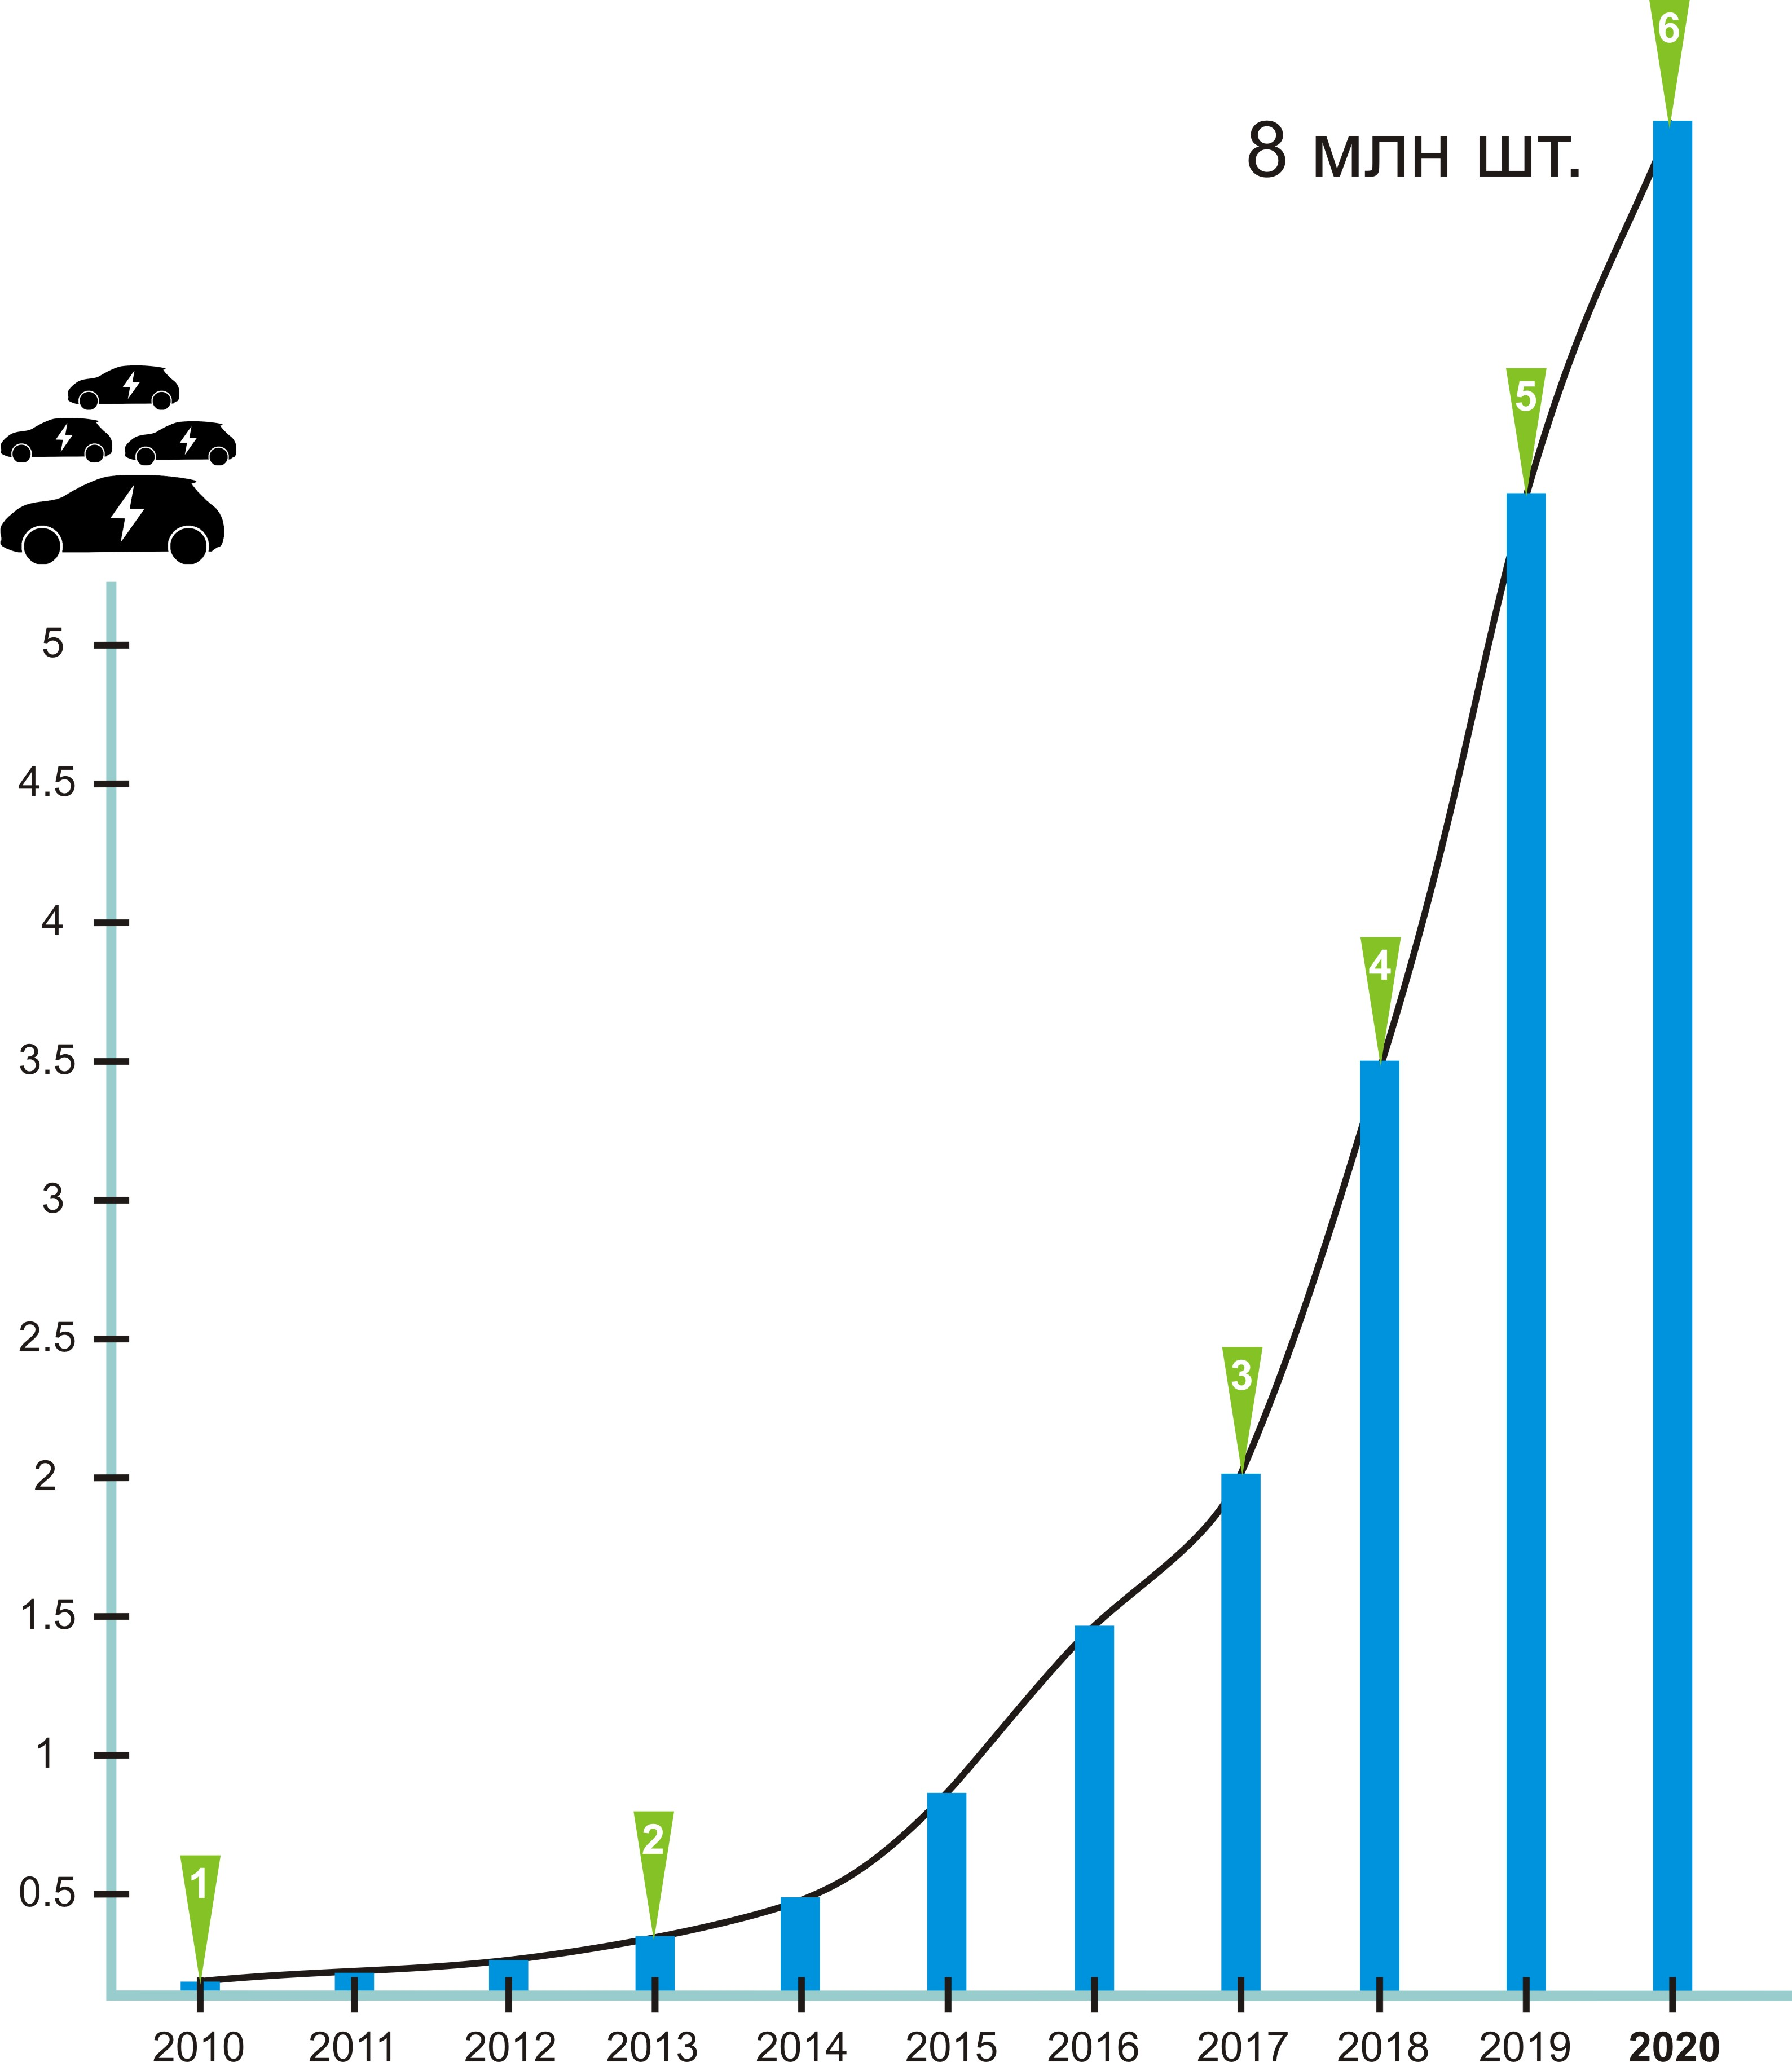
\includegraphics[width=12cm]{chart1}
\vspace*{1cm}

\begin{enumerate}
	\item Начало выпуска первого массового электромобиля в современной истории - Nissan Leaf
	\item Начало выпуска Tesla Model S
	\item Начало выпуска Tesla Model 3
	\item Каждый третий автомобиль в Норвегии электрический
	\item Количество зарядных станций в Европе превысило количество АЗС
	\item Количество проданных электромобилей Tesla превысило 1 млн штук
\end{enumerate}



\vspace*{1cm}
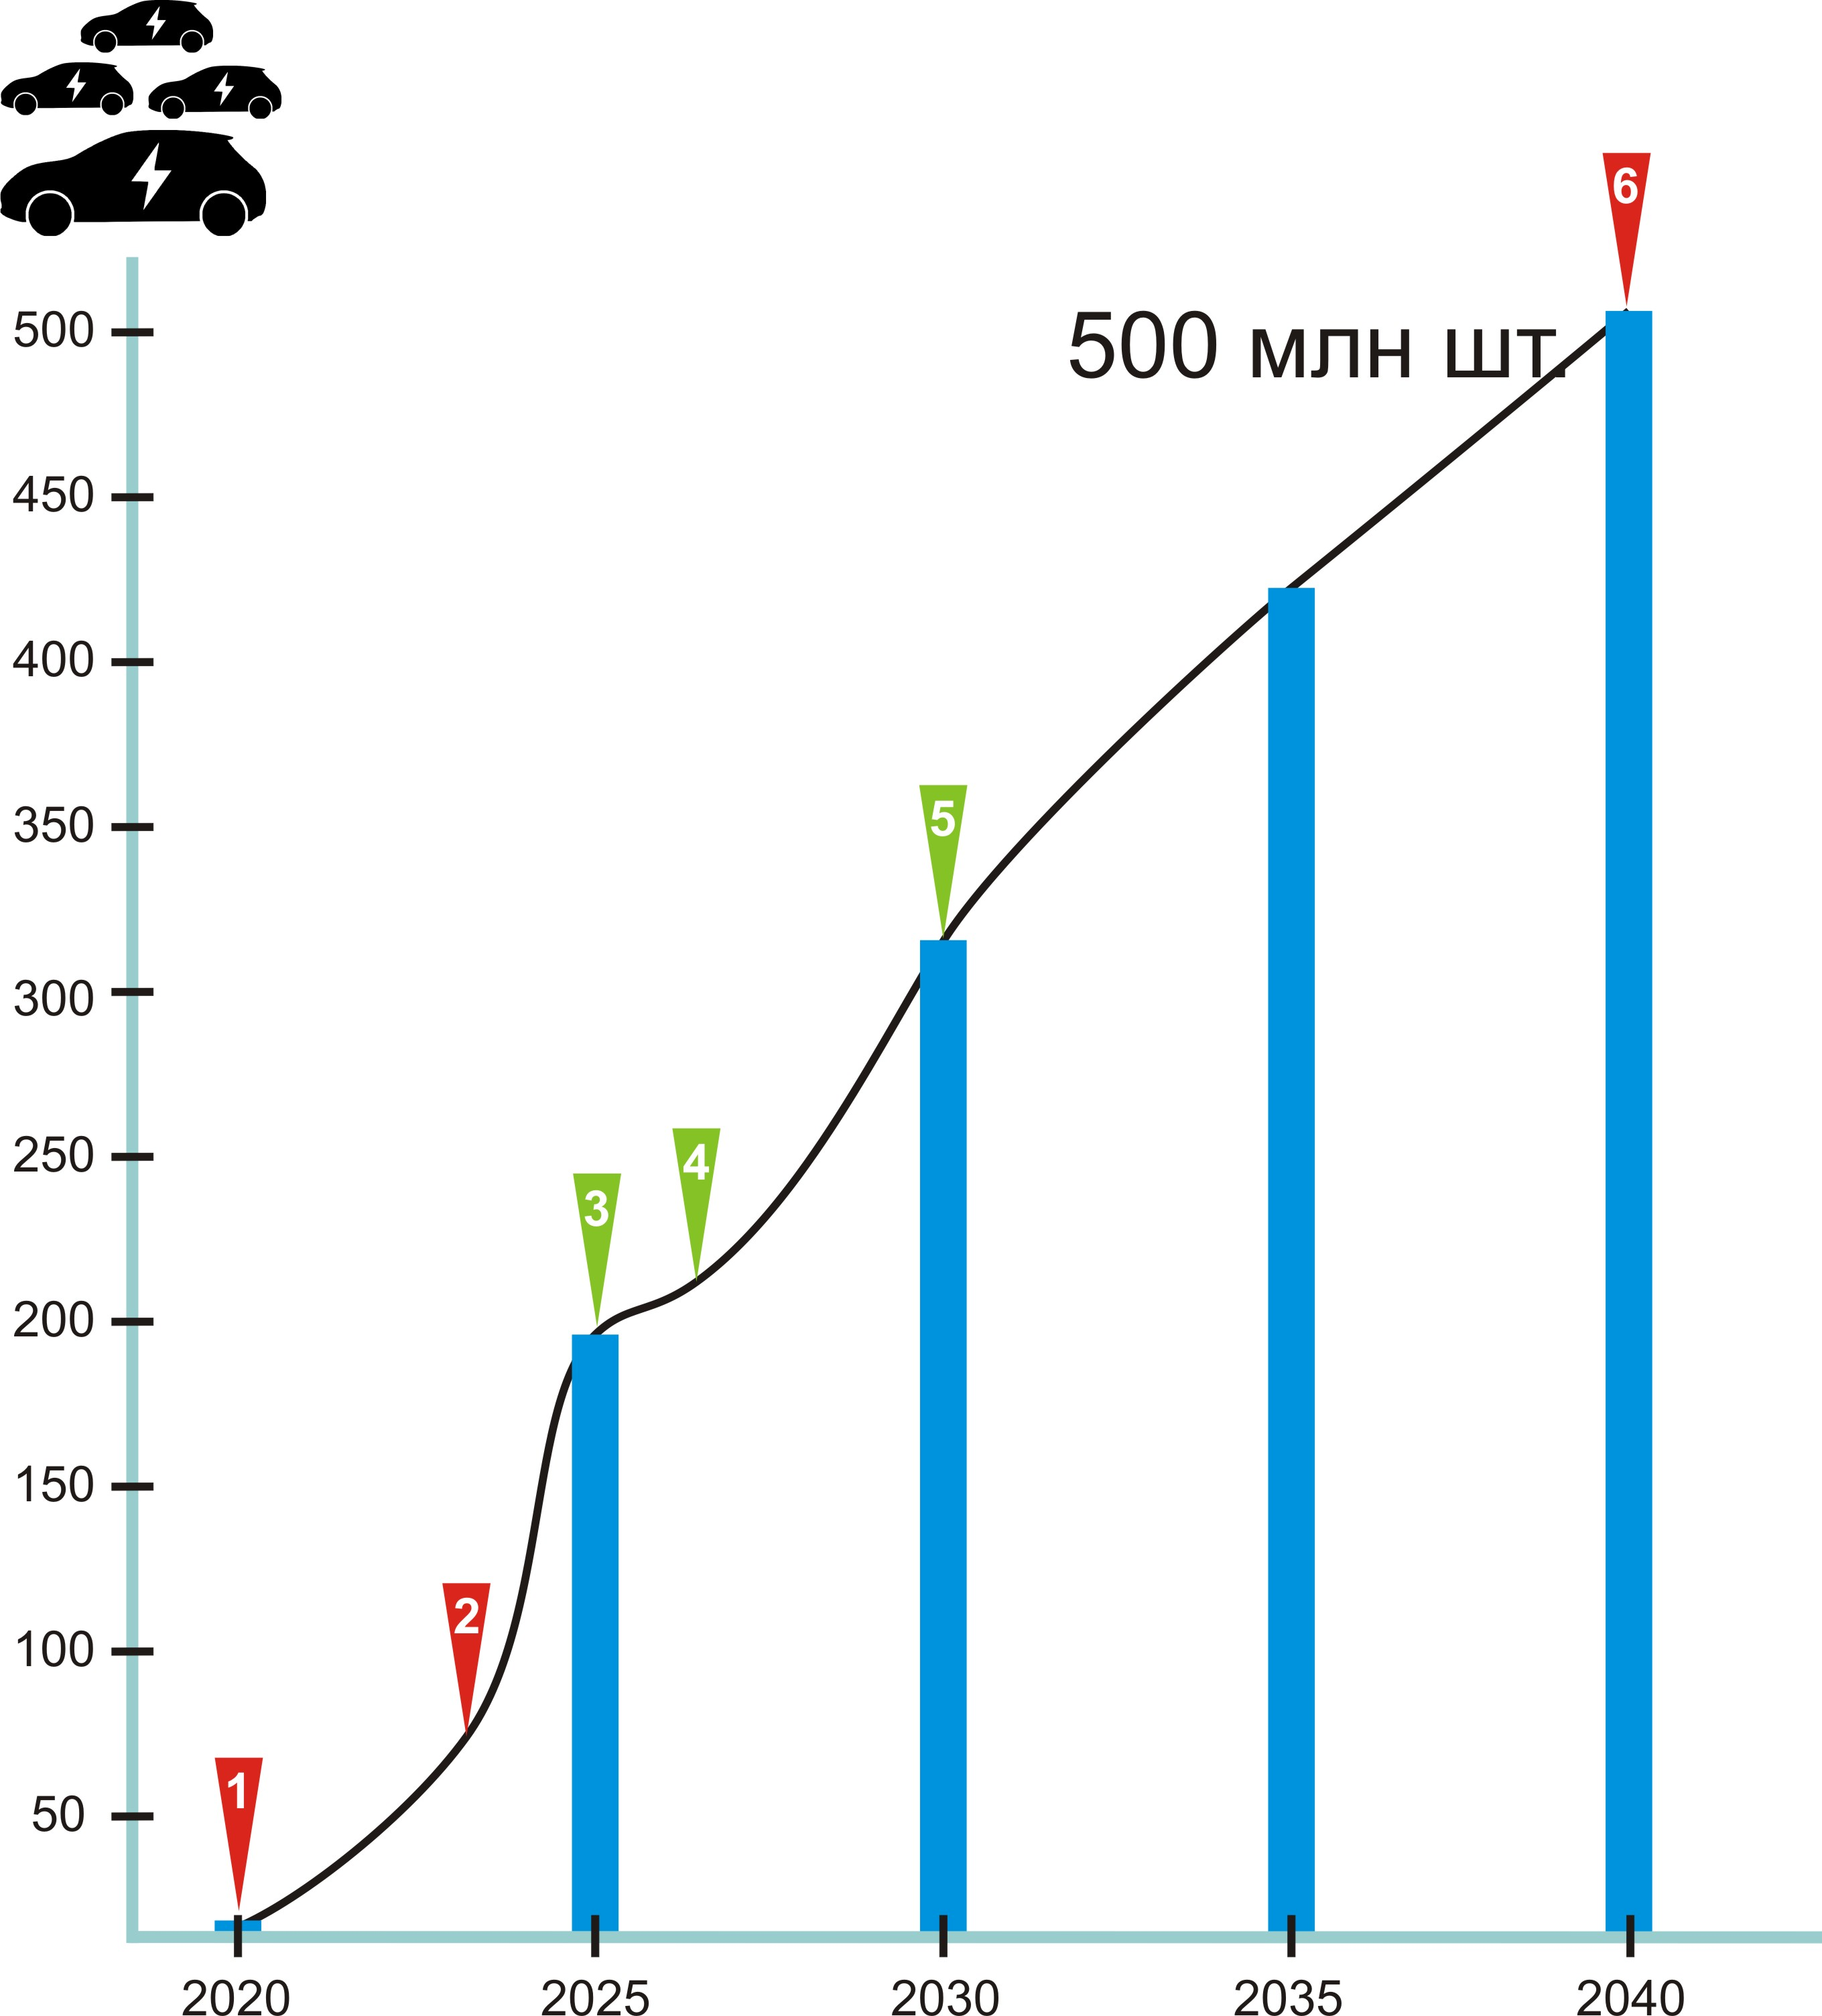
\includegraphics[width=12cm]{chart2}
\vspace*{1cm}

\begin{enumerate}
	\item Отказ от дальнейшей разработки в области ДВС крупнейших автопроизводителей, таких как BMW, Mercedes, Volvo, Audi, Volkswagen, Toyota
	\item Выравнивание стоимости электромобиля и автомобиля на ДВС (обусловлено снижением стоимости аккумуляторов)
	\item Начало распространения беспилотных, коммерческих электромобилей
	\item Toyota и Volkswagen прекращают выпуск автомобилей на ДВС
	\item Запрет эксплуатации ДВС в Голландии, Швеции, Шотландии, Дании и Израиле
	\item Полный запрет ДВС в Европе
\end{enumerate}


Какой вывод можно сделать из приведённых данных? Мы находимся на заре новой эры автотранспорта. Во всех развитых странах полным ходом идёт переход на электромобили, и это уже не просто фантазии отдельно взятых энтузиастов, это конкретные планы крупнейших автомобильных гигантов. 

Однако, светлое будущее не наступит само по себе. Его необходимо построить. 

\section{Электромобили в России}
На момент августа 2021 года, например, в нашей стране на сегодняшний день всего около \textbf{500} полноценных зарядных станций. Чтобы понять, какое будущее ждёт электромобили при таком раскладе, нужно посмотреть на автомобили с ДВС через эту призму. Вы бы захотели приобретать авто, заправить которое можно было бы только в 500 точках на всю Россию? Которые, вдобавок, должным образом не обслуживаются, и внятных перспектив развития которых не предвидится. Наверное, нет. И это логично, поскольку автомобиль покупают не для самоистязания, а чтобы увеличить степень личной свободы и повысить комфорт передвижения. Поэтому неизбежным условием для увеличения количества электромобилей и их \textbf{комфортной} эксплуатации, является \textbf{развитие инфраструктуры}. 

\section{Проблематика инфраструктуры}
Помимо недостаточного количества самих станций, большинство из тех, что есть в нашей стране, расположены в самых странных и неудобных для автовладельца местах. А также не имеют должного обслуживания и адекватной информационной поддержки. В основном эти станции принадлежат гос. компаниям со всеми вытекающими.

Такое положение дел формирует “порочный круг”. Малое количество электромобилей делает идею развития зарядной инфраструктуры неинтересной для бизнеса. В свою очередь, отсутствие инфраструктуры значительно тормозит рост количества электромобилей. 

Решить проблему, по идее, способно государство, потому как у него достаточно ресурсов и инструментов. Наше государство пытается что-то делать (выпускаются законы, облегчающие финансовую нагрузку на владельцев электромобилей, адаптируются разрешительные акты, регулирующие установку зарядных станций, закупаются и устанавливаются бесплатные зарядные станции в городах и на трассах), но в масштабах страны эти усилия пока что незаметны. 

В 2016, когда мы только начинали, при слове “электромобиль” на нас смотрели, как на городских сумасшедших. И тогда действительно было рано для инвестирования в это направление по целому ряду факторов, главный из которых - рынка как такового еще не было. 

Однако сейчас рынок уже есть и самое время его осваивать.  


\chapter{Рынок России и перспективы бизнеса}

\section{Количество электромобилей}

Согласно данным аналитического агентства Автостат, в РФ количество зарегистрированных электромобилей в 2019 \href{https://www.autostat.ru/news/38371/}{было} 3.6 тысяч, в 2020 \href{https://www.autostat.ru/news/42999/}{было} 6.3 тысячи, и по данным Автоньюз, в 2021 \href{https://www.autonews.ru/news/602002889a7947acbb3fd189}{почти} 11 тысяч. По различным данным доля незарегистрированных электромобилей составляет еще от 25 до 40\% Данные для статей взяты из базы ГИБДД, поэтому мы можем считать их объективными. 

Тенденция роста почти 90\% в год, учитывая полное отсутствие инфраструктуры и пандемию.

Исходя из опыта общения с владельцами электромобилей и участия в огромном количестве различных мероприятий по теме, мы с уверенностью можем сказать, что количество потенциальных покупателей в десятки раз больше. Многие люди прямым текстом говорят: “когда появится возможность нормально эксплуатировать электромобиль, я сразу же его куплю”. Т.е. нас ожидает бум интереса к электромобилям, когда появится более-менее адекватная зарядная инфраструктура. 

\section{Потенциальный объём рынка зарядных станций}

Весь рынок РФ мы разбили на сегменты. Каждый сегмент мы рассматривали с двух позиций. Насколько вероятно в ближайшее время формирование потребности в станциях и потенциальный объём. 

\subsection{АЗС}

Со слов вице-президента НТС Дмитрия Гусева в РФ более 23 000 АЗС. 60\% из которых независимые. 

На АЗС целесообразно ставить только станции постоянного тока.

Мы пообщались с представителями всех крупнейших компаний на рынке по вопросу установки станций на их заправках. В целом, идея установки им интересна, и некоторые компании уже пробовали устанавливать станции и собирать статистику. Как только количество электромобилей увеличится, и станции станут рентабельными, они начнут ставить зарядные станции за свой счёт. 

\subsection{Строительные объекты}

По данным Минстроя на февраль 2021 года зарегистрировано 3109 застройщиков, и выдано 5568 разрешений на строительство.

На 21 год запланирован ввод в эксплуатацию 40 726 тыс м2 - 796 000 квартир по всей стране. 

Согласно постановлению правительства РФ от 29.12.2009 необходимо обеспечивать минимальное количество парковочных мест 1.6 шт на 1 квартиру. Таким образом на 796 000 квартир, ожидаемых для ввода в эксплуатацию в 21 году, должно быть обеспечено 1273600 парковочных мест, и в соответствии с РДМ-32-28-2018 3\% из них должны быть оборудованы зарядными станциями для электромобилей (38 208 шт)

Из расчета на 1600 м2 1 станцию (из новой редакции петербургских Правил землепользования и застройки (ПЗЗ)), получается 25 454 станции по идее может быть поставлено в новостройках уже в 21 году.

\subsection{Гостиницы и отели}

Согласно \href{https://классификация-туризм.рф/displayAccommodation/index}{данным} Федерального агентства по туризму в России 14940 гостиниц и иных объектов размещения. 

Отели напрямую заинтересованы в установке станций, поскольку наличие такой станции уже сейчас даёт баллы в наиболее популярных приложениях букинга. 

\subsection{Трассы}

Из соображений удобства рационально ставить 1 станцию постоянного тока каждые 50 км дороги. На трассах целесообразно устанавливать только сверхбыстрые (от 100 кВт) станции постоянного тока. 

Всего протяженность трасс, где в принципе имеет смысл размещать зарядные станции  - 63 290 км (1265 шт)

\subsection{Малый и средний бизнес, торговые точки, бизнес-центры}

Владельцы любых коммерческих помещений могут покупать зарядные станции и с помощью приложения монетизировать. По сути станция будет работать, как вендинговый аппарат, генерируя небольшую прибыль с продажи электричества, как рекламный щит (модели с экраном) привлекая электромобилистов, и тем самым повышая продажи основных услуг бизнеса. 

Как видно, с увеличением количества электромобилей, нас ожидает бум интереса к зарядным станциям. 

Зарядная инфраструктура и электромобили являются частями одного целого, и рассматривать их отдельно не имеет смысла. И соответственно, усилия наиболее целесообразно вкладывать сразу в обоих направлениях.  

Сценарий развития рынка вполне очевиден. 

Увеличение количества различных моделей электромобилей и их удешевление (за счет конкуренции и развития аккумуляторной химии) с одной стороны и постоянное и неизбежное подорожание бензина с другой, будут стимулировать темпы прироста количества электромобилей. 

Растущую потребности в зарядных станциях всё больше будет привлекать компаний и частных предпринимателей к развитию инфраструктуры. Точечно поставленные станции будут генерировать всё большие прибыли, и их количество будет неизбежно расти. 

К определенному моменту количество зарядных станций достигнет точки, когда эксплуатация электромобилей станет в целом удовлетворительной, и на первый план в принятии решения о переходе на электротранспорт выйдет экономическая выгода от его использования. Информация об этом распространится в инфополе и всё больше людей начнут задумываться о покупке электромобиля.

Это резко увеличит потребность в электромобилях. На растущий спрос рынок ответит ростом предложения. Всё больше компаний начнут заниматься привозом и продажей электромобилей. 

Рост оборота капитала рано или поздно привлечет в сферу электротранспорта крупных игроков, и начнется масштабное развитие по всей стране.

Чтобы иметь адекватные шансы на конкурентную борьбу с крупными компаниями, к моменту, когда пойдёт ажиотаж нужно уже быть полностью готовыми: иметь качественный продукт, налаженное производство, отлаженную логистику и средства коммуникации с клиентом и приличный доход. 

Ждать, когда произойдёт взрыв и только потом начинать - значит остаться у обочины и наблюдать, как рынок съедают корпорации.

Рынок будет сформирован и полностью занят. Это неизбежность технологического развития общества. Открытым остаётся вопрос - какие конкретно игроки успеют зайти на этот рынок и получить долю. Мы уже в их числе. Тоже хотите? Тогда добро пожаловать в сообщество. 

Однако, сказать, что мы получим свою долю рынка - это одно. А вот реально её получить - совсем другое. Для того, чтобы слова превратить в результат, нужно понимание что делать, необходимые инструменты и люди, которые сделают то, что нужно. 


\chapter{Стратегия освоения рынка}

\section{Подготовительный этап}
\subsection{Продукт}

Любой бизнес начинается с качественного, конкурентоспособного продукта. 

Один из наших основных продуктов - это услуга по зарядке электромобилей. Для реализации практической функции - непосредственной зарядки автомобиля - нам необходимо соответствующее техническое устройство - зарядная станция. 

Поскольку потребитель нашего продукта человек, помимо технических характеристик, важным свойством зарядной станции является дизайн. Наш дизайн - это одно из конкурентных преимуществ, роль которого будет возрастать по мере развития рынка и появления всё большего количества производителей. Станция должна выглядеть стильно, аккуратно и привлекать внимание. 

Другое свойство, обязательное для конкурентоспособного продукта, это удобство взаимодействия. Наша задача сделать практическое использование станций интуитивно понятным, комфортным и стабильным. Для этого мы разработали мобильное приложение. Также в долгосрочной перспективе приложение это мощнейший инструмент коммуникации с пользователями и соответственно серьезное конкурентное преимущество. Приложение уже можно скачать для Android и IOS. Функционал будет расширяться и в конечном итоге приложение станет одним из ключевых инструментов внутренней коммуникации, объединяющим все наши продукты. 

Услуга по зарядке электромобилей - продукт комплексный и сложный. Чтобы на выходе получилось необходимое качество, все его элементы должны быть созданы профессионалами и должны управляться профессионалами. 


\subsection{Команда}

На момент Августа 21 года, команда Portal Energy составляет 24 человека (выросла с 7 человек). У нас есть:
Команда управления, 
команда инженерной разработки, 
команда разработки софта, 
производственная команда,
команда дистрибуции. 

Количество человек будет расти по мере увеличения количества задач. 

Как уже говорилось, Portal Energy это сообщество заинтересованных людей, что значит, любой член сообщества является частью команды. Мы рассчитываем привлекать участников сообщества к деятельности компании, когда для этого будут разработаны необходимые инструменты.

\subsection{Независимость и гибкость}

В современном мире производство, как правило, распределено. Крупнейшие компании закупают компоненты у разных производителей и уже из них собирают свой конечный продукт. 

Мы, разумеется, тоже рассматривали данную модель. Но быстро от неё отказались. Специфика российского рынка делает международную логистику крайне дорогой и уязвимой к накладкам по времени. Что мы позволить себе не можем, потому как в случае с перебоем комплектующих мы сразу же нарушаем все договоренности по срокам с клиентами. В долгосрочной перспективе с такой уязвимостью рассчитывать на успех в конкурентной борьбе, как минимум, наивно. 

Второй вопрос - это вопрос гибкости. Разработка технологических устройств предполагает длительную отладку и постоянное усовершенствование определенных узлов и элементов. Оперативно получить необходимые комплектующие для тестов имея поставщика за океаном - невозможно.

Таким образом мы пришли к неизбежности собственной разработки всех комплектующих и написания софта. 

На сегодняшний день мы сами разрабатываем платы контроллеров, сами пишем для них ПО. Мы сами производим корпуса и производим сборку станций. Единственные звенья, которые пока что являются импортом - коннекторы и выпрямители тока. Однако, и их производство мы ближайшее время наладим на территории России. 

\section{Этап отладки и подготовки к масштабированию}

\subsection{Производство} 

Итоговый вариант производства, который мы хотим видеть - производство полного цикла. На вход поступает металлопрокат и комплектующие электроники, на выходе получается полностью готовая к работе зарядная станция. 

Такое производство мы будем создавать в два этапе. 

Первый этап - экспериментальная лаборатория с малой производственной мощностью - до 50 станций в месяц. 
Второй этап - производство полного цикла с мощностью от 1000 станций в месяц. 

На текущий момент мы полностью реализовали производство первого этапа с мощностью 40 станций в месяц и перспективой её приращения до 100 штук в месяц. Производство расположено рядом с офисом разработчиков, что позволяет нам комфортно и оперативно реализовывать изменения и исправлять ошибки, найденные в станциях, поступивших в эксплуатацию.

Второй этап мы начнём, когда весь запланированный модельный ряд будет отлажен и инфраструктурный проект будет способен загрузить производство хотя бы на 100 + станций в месяц. И постепенно наращивать мощность.

Таким образом к моменту начала ажиотажа мы планируем иметь производство с мощностью от 1000 станций.

О старте привлечения инвестиций мы сообщим на наших информационных ресурсах. Поэтому если вам интересна идея инвестирования в производство, следите за новостями. 

\subsection{Инфраструктурный проект}

Как было видно из данных о состоянии рынка и количестве электромобилей, наиболее рациональная стратегия - работа в обоих направлениях параллельно.

Сейчас в инфополе нет никакой активности вокруг темы электротранспорта, и у людей, которые являются нашими потенциальными клиентами, сформировано однозначное понимание - в России зарядной инфраструктуры нет и не предвидится. Поэтому первая задача - сформировать интерес к теме электротранспорта, создать движение информации и показать Portal Energy, как авангард в вопросе развития зарядной инфраструктуры.

Это сформирует у людей запрос на покупку электромобилей. Поскольку сейчас купить хороший электромобиль по адекватной цене в России практически невозможно, наша вторая задача - удовлетворить спрос на электромобили. 

Рост количества электромобилей сформирует потребность в увеличении количества зарядных станций. Т.е. наши потенциальные клиенты станут реальными. И следовательно, третья задача - удовлетворить спрос на зарядные станции.

Наш инфраструктурный проект - это и есть работа над всеми тремя задачами. 

Двое членов команды, Петр Мовчан и Александр Павлов совершили автопробег на “Тесле” из Санкт-Петербурга до Владивостока. По пути следования мы устанавливали зарядные станции. По итогу поездки мы поставили 17 станций по всей стране, сформировав “Путь Света” (по названию нашей главной модели “Light Way”), по которому подобную поездку сможет повторить любой желающий с подходящим электромобилем. 

Нам важно было обкатать процедуру установки и дистанционной отладки станций как в ближайших к Петербургу городах, так и в местах до которых тысячи километров. Так же поездка стала важным этапом исследования рынка. Мы получили эмпирические данные того, как обстоят дела в разных регионах России в сфере электротранспорта, наладили контакты с администрацией и местными электромобилистами. 

Практика показала, что бессистемное распространение зарядных станций даст слишком отсроченный эффект и, в условиях ограниченных ресурсов, контрпродуктивно. Потому как одна-две станции даже на небольшой город не повлияют существенно на комфорт эксплуатации электромобиля, более того, загрузка этих станций будет минимальна долгое время. И учитывая огромные размеры нашей страны, прежде чем инфраструктура начнёт окупаться, могут пройти годы. И с таким подходом, мы, скорее всего, не успеем набрать достаточный вес к моменту начала ажиотажа. 

В качестве решения мы разработали модель комплексного подхода к развитию инфраструктуры. Вместо точечного распространения станций по всей стране, мы выбираем город, устанавливаем там достаточное количество зарядных станций, запускаем электротакси, организуем привоз и продажу электромобилей и открываем сервис. 

Таким образом мы создаём полноценную систему, которая сможет удовлетворить все потребности людей, решивших приобщиться к теме электротранспорта. Установленные по всему городу зарядные станции решат вопрос с зарядкой на начальном этапе. По мере увеличения количества электромобилей мы будем устанавливать дополнительные станции, но комфорт эксплуатации будет достигнут сразу. Электротакси позволит людям познакомится с электромобилями, наглядно продемонстрирует плюсы их эксплуатации, обеспечит загрузку зарядных станций и будет приносить прямой доход в систему. Реализованная через партнеров возможность взять электромобиль в лизинг, или trade-in значительно упростит переход с ДВС. Администрации города крайне выгоден такой подход, потому как они закрывают одну из актуальных своих задач, и потому мы можем рассчитывать на сотрудничество и содействие в получении наиболее привлекательных мест под установку станций. 

Все необходимые компетенции, инструменты и договоренности у нас уже есть. Ближайшее время мы начнем подготовку пилотного города. 

Мы считаем, что лучше всего управлять и развивать федеральную сеть зарядных станций и электротакси смогут те, кто будет ими пользоваться. То есть, вы. Но чтобы вам это было интересно, вы должны получать с неё доход. 

Для этого мы разработали инвестиционную модель. 





\chapter{Инвестиционная модель}
Поскольку подобная задача может быть решена только в условиях абсолютного доверия участников сообщества друг к другу, мы обязаны были это доверие сформировать. По нашему мнению, лучшим фундаментом в формировании доверия является полная прозрачность всех финансовых процессов в организации. И для обеспечения такой прозрачности, мы выбрали \textbf{блокчейн}. 

Сейчас мы имеем 2 токена которые являются разными сторонами одной экономики, где
токен POE и его экономика отвечает за зарядные станции, а токен tPOE отвечает за развитие электро-такси в конкретном городе. В итоге мы получим здесь и сейчас плановую загрузку станций, а электро-такси получает безболезненную эксплуатацию автомобилей за счет развитой инфраструктуры. 

Начинаться все будет с формирования проекта, который будет в себя включать следующую информацию:

\begin{enumerate}
	
	\item город развития
	\item задача проекта, ценность для сети
	\item качество дорог
	\item кол-во проживающих людей 
	\item лояльность местной администрации, места, тариф, техническая возможность, договор!
	\item местный бизнес который будет помогать реализовывать проект, иметь договор
	\item площадь города
	\item минимальное необходимое кол-во станций и их конфигурация
	\item минимальное кол-во электромобилей, модель, марка, запас хода, обоснованность выбора автомобиля
	\item согласованная территория для поддержания таксопарка
	\item список, кол-во стоимость запасных деталей для автомобилей
	\item юридическое лицо которое будет владеть станциями и автомобилями
	\item экономические расчеты, показывающие срок окупаемости проекта 
	\item сколько нужно денег на зарядную инфраструктуру
	\item сколько нужно денег на электро-такси
	\item риски 20\% (возможные дополнительные работы и их стоимость)
	\item этапы выполнения работ и стоимость каждого этапа
	\item срок сбора средств
	\item ответственное лицо которое будет реализовывать проект

\end{enumerate}
 
\section{Логика реализации проекта}

\subsection{Этап 1: Инициация проекта}
	Человек, который хочет предложить проект в систему, должен сформировать заявку в соответствии с вышеизложенными пунктами. 

\subsection{Этап 2: Верификация сообществом}
	Сформированная заявка размещается на форуме, где её смогут проанализировать участники сообщества и высказать свои замечания и предложения. Это даст возможность инициатору удостовериться, что на следующем этапе проект будет одобрен.

\subsection{Этап 3: Голосование}
	После того, как инициатор убедился, что у сообщества нет претензий к его проекту, он размещает заявку в блокчейне на голосование. Для предотвращения  спама бессмысленных или недоделанных проектов в систему, за размещение будет взыматься стоимость. В случае успешного голосования стоимость размещения переходит в залог.

\subsection{Этап 4: Назначение ответственного за проект}
	По умолчанию инициатор предполагается как лицо, ответственное за весь проект. В случае, если инициатор по какой-либо причине не может выполнять роль ответственного, ему необходимо указать кто будет выполнять эту роль. Чтобы проект перешел к следующему этапу "Сбор средств" ответственное лицо должно внести залог (застейкать usdt на смарт-контракт) равный стоимости самого дорогого этапа проекта.

\subsection{Этап 5: Сбор средств}
	Сбор средств начинается с момента завершения предыдущего этапа. Длительность данного этапа указывается в заявке на этапе голосования. Люди вносят средства на смарт контракт, система резервирует для них соответствующее количество токенов POE и tPOE (по курсу на момент сбора средств). Как только собирается 80\% от общей стоимости проекта, у ответственного лица появляется возможность перевести его на следующий этап "Выполнение работ". Если средства собраны на 100\% у ответственного есть 5 дней, чтобы взять проект в работу. Если этого не происходит, проект отменяется, средства возвращаются, а ответственное лицо штрафуется на 10 \% суммы залога, и его репутация страдает. 

\subsection{Этап 6: Выполнение работ}
	Как только проект переходит в этот этап, система распределяет токены POE и tPOE среди инвесторов. После этого вернуть средства через механизм отмены проекта уже невозможно. (Инвестор по желанию может продать свои токены по текущему курсу внутри DeFi). 

	Работы по проекту выполняются в соответствии с этапами и принимаются в систему итерационно. 
	
	Процесс принятия работ по этапу:
	\begin{enumerate}
		\item После выполнения конкретного этапа ответственное лицо помечает его, как "выполнено" и предоставляет все факты, подтверждающие успешное выполнение работ.
	    \item Сообщество принимает работы путём голосования.
	    \item Следующий этап начинается только если голосование за предыдущий считается завершенным, а если этап был последним, весь проект переходит в статус "Завершено".
	\end{enumerate}

\subsection{Этап 7: Выплата вознаграждений}
	После принятия работа по последнему этапу, проект считается завершенным, и происходит автоматическое начисление вознаграждения ответственному лицу в виде доли от общей стоимости проекта. Токены вознаграждения активируются из общего пула эмиссии. 



Так будет происходить реализация всех проектов, за исключением пилотного, который будет происходить на доверии к PortalEnergy 




\section{Эмиссия и распределение токенов}

Токен POE имеет эмиссию в \textbf{10 000 000 POE}, эмиссия не может быть увеличена, так сложилось исторически.
 
Токен tPOE имеет \textbf{динамическую эмиссию}, токены выпускаются в нужном количестве как только проект достигнет шестого этапа.

Каждый раз когда токены выпускаются, 42.8\% от активируемых токенов идёт на счёт компании, в результате после продажи 7 000 000 токенов, за компанией останется 3 000 000. Такая логика позволит нам всегда перераспределять ровно 30\% от общего объёма команде Portal Energy.

Описанная модель позволит нам сделать инвестирование привлекательным на любом этапе, т.к. доход от инфраструктуры инвестор начнет получать сразу после установки станций. 

\section{Фонд развития и поддержки}
\label{storage}
Для того чтобы поддерживать уже созданную инфраструктуру и развивать текущую без вливания новых инвестиций.
Процент от дохода станций остается на смарт контракте распределения токена, на момент старта это 20\%, этот процент потом можно будет менять путем голосования держателями токенов. 

\section{Распределение доходов}
\label{capital}
Раз в период денежные средства будут переводиться в криптовалюту Ethereum на смарт-контракт PortalEnergyDistributor который отвечает за распределение средств в нужном процентном соотношении, по токенам которые застейканы на смарт контракт.

\textbf{Пример для токена POE, дано}:

\begin{itemize}
	\item продано инвесторам в кол-ве 300 000 POE
	\item распределено команде PortalEnergy 128 400 POE
	\item токенов участвующих в распределении 428 000 POE
	\item установленно станций 70 штук с общим условным минимальным месячным доходом в 10 000\$
	\item курс ether к доллару условно 400\$,  на кошелек распределения уходит 25 ether в месяц
\end{itemize}

\textbf{Распределение:}

\begin{enumerate}
	\item Контракт получает на входе ether в размере 25 единиц.
	\item 20\% идет в фонд развития и поддержки инфораструктуры
	\item Получаем кол-во ether на каждый токен: 20/428 000 = 0,000046729
	\item Получаем список держателей токенов
	\item По очереди берем каждого держателя токена, определяем кол-во токенов у держателя и умножаем на кол-во эфиров, т.е. Если адрес имеет 2000 токенов, то: 2000*0,000046729 = 0,093457944 ether
	\item Умножаем на курс эфира 400*0,093457944 = 37\$ в мес или 444\$ в год, что равно примерно 24\% годовых. 
\end{enumerate}


24\% годовых это начальный и минимальный процент исходя из текущего состояния рынка, когда каждая зарядная станция используется только на 25\%. С ростом кол-ва электромобилей в стране резко увеличится и доход со станций.  

Периодичность распределения будет меняться в зависимости от объёма распределяемых средств. Чем больше объём распределяемых средств, тем чаще будут выплаты. Порог частоты - 2 раза в месяц. Такая модель позволит минимизировать расходы на обслуживание транзакций.

\subsection{Доходность зарядных станций}

Доходность всей сети зависит от того, сколько стоит киловатт энергии, продаваемой через станции и количества проданных киловатт. Киловатты станций переменного и постоянного тока стоят разных денег и поэтому считаются отдельно. 

Также важно учитывать, что одна и та же станция может генерировать разный доход. Это зависит от места, где станция расположена.

Формула расчета годового дохода простая: X * Y * Z * A 


Где:
\begin{enumerate}

	\item Х - стоимость киловатта (имеется в виду чистый доход, т.е. тариф станции минус тариф энергокомпании, минус операционные расходы)

	\item Y - сколько киловатт может продать станция в час (Переменный ток: коннектор тип1 - 9, коннектор тип2 - 22. Все наши инфраструктурные станции оборудованы обоими коннекторами, т.е. минимальное количество - 9, максимальное 31. Постоянный ток - заявленная максимальная мощность. Т.е. 40, 60, 80 и т.д. Если подъезжает несколько машин, мощность распределяется равномерно и не может превышать максимальную)

	\item Z - количество часов, которое станция работает в сутки (может быть от 0 до 24)
	\item A - количество рабочих суток в году 
\end{enumerate}

Как правило, стоимость коммерческого тарифа - 7 рублей. Средняя прибыль (исходя из практики тех, кто уже монетизирует купленные в собственность станции) на киловатт 5-8 рублей на станциях переменного тока и 8-15 рублей на станциях постоянного тока. 

Вся реальная статистика будет режиме онлайн находиться на нашем сайте. Мы не будем приводить тут математику различных сценариев, ведь, как уже было сказано, одна и та же станция может приносить доход отличающийся в десятки раз (если станция в удобном, “проходном” месте, она будет занята большую часть суток каждый день). Всё зависит от места её расположения.

Но если вам всё-таки интересно, то самый пессимистичный сценарий (станция работает 1 час на тип1 в день) наш “Спутник” будет приносить 8\% годового дохода. При самом оптимистичном сценарии (станция работает 24 часа на обоих коннекторах) этот же “Спутник” будет приносить 678\% годового дохода.


\subsection{Доходность с такси}

Формула доходности:

A - Чистая прибыль с поездки (цена, минус комиссия агрегатора, минус доля водителя, если машина сдаётся в аренду)
B - Количество поездок за отчетный период
C - Стоимость полной зарядки (по сути 2 вариант - на постоянном и переменном токе)
D - Количество полных зарядок на отчетный период
E - Стоимость амортизации


(A * B) - (C * D) - E

Так же как и в случае с доходностью зарядных станций, мы не будем просчитывать конкретные сценарии и приводить цифры, поскольку, они тоже могут отличаться в разы. 
Мы не видим смысла завышать, или занижать ваши ожидания. Всё будет видно, когда мы получим данные после реализации пилотного проекта.

Однако, несколько слов о том, за счет чего формируется наша уверенность в успехе, сказать стоит. 

На сегодняшний день рынок такси достаточно развит, и конкуренция там весьма серьезная. Для того, чтобы рассчитывать на успех, необходимо либо иметь огромный капитал, либо иметь значительное конкурентное преимущество. В нашем случае главное конкурентное преимущество - электромобили.
Если брать доходность такси, основными статьями расходов будут стоимость топлива и амортизация автомобиля. И именно по этим двум показателям электромобили значительно выгоднее ДВС.
Главная проблема электромобиля сегодня - отсутствие зарядных станций. Во-первых, необходимость их включать в стоимость бизнеса, существенно её увеличивает. Плюс, для реализации (приобретения, установки и обслуживания) нужны специальные компетенции. И если мы говорим о такси, как бизнесе, специалисты по обслуживанию зарядных станций - еще одна статья расходов.
Поэтому при всей очевидной выгоде подавляющее большинство компаний и предпринимателей предпочитают не связываться с электромобилями, а делать по понятной и проверенной схеме. 
В нашем случае все необходимые компетенции у нас есть. И таким образом из проблемы, которую надо решать, зарядные станции превращаются во второе наше ключевое конкурентное преимущество. 
Поэтому для нас проект с установкой зарядных станций в отдельно взятом городе и запуске электротакси является не сложным и рискованным предприятием с множеством неизвестных переменных, а понятной и выгодной схемой.


\chapter{DAO}

Любой уважающий себя блокчейн проект имеет такую форму управления ( \ref{dao} ). Сейчас устоялась практика логики голосования такая: один токен = один голос. На наш взгляд это в корне неверная логика, так как особо обеспеченные люди могут скупать большее кол-во токенов и очень сильно влиять на результаты голосования. Поэтому мы сформировали свои правила.

\section{Правила}

Основные правила

\begin{itemize}
	\item один человек имеет только один голос.
	\item можно изменить голос до окончания голосования
	\item можно создать второе голосование отменяющее первое, в голосовании действуют те же правила
	\item токены на адресе или стейке должны быть не менее 30 дней чтобы иметь права голоса
	\item один голос считается если у человека от 200 токенов до бесконечности, так же принимается сумма токенов POE и tPOE которые будут так же являться одним голосом
	\item в голосовании участвуют только те, на кого непосредственно будут влиять результаты голосования.
	\item участвуют только те, кто указал свои компетенции, компетенции надо обновлять раз в пол года иначе участник выпадает из кворума.
	
\end{itemize}


\section{Компетенции-интересы}
Каждый участник который хочет участвовать в DAO должен будет указать в каких сферах он имеет компетенции или интерес, допустим человек разбирается в электрике, знает хорошо какие то города, программирует и т.д.

Эти данные нужны для расчета кворума и не являются решающим фактором в голосовании.  т.к. даже если мы подтвердим каким то образом компетенцию человека, то мы не можем гарантировать то что он будет голосовать в интересах общества

\section{Кворум}
	
Очень важный параметр в голосовании, здесь мы делим голосования на 2 понятия:

\subsection{Параметры смарт контрактов}
Все параметры смарт контрактов, такие как параметр процента отчислений в фонд развития и поддержки \ref{storage} затрагивают интересы всех участников сети, соответственно кворум в будет считаться набранным если участвуют 80\% людей. 

\subsection{Проекты}
Основную нагрузку в голосовании будут создавать проекты. Вопросов для голосования будет очень много и мы понимаем что никто не будет голосовать всегда по всем вопросам. Поэтому создавая проект человек должен указать список компетенций-интересов которые будут затронуты проектом, и исходя из этого списка будет формироваться список участников которые могут голосовать в проекте. 

С такой логикой мы сможем создать приложение для голосования где будет поток голосований только по интересующим вам темам. 

\section{Варианты ответа и принятие решения}

\begin{itemize}
	\item Согласен
	\item Против
	\item Не знаю
\end{itemize}

По итогу голосования мы будем иметь следующие результаты,  пример:\par

Кворум считается набранным если есть 1000 голосов

\begin{itemize}
	\item Набрано голосов 1025
	\item Согласны - 200 человек
	\item Против - 300 человек
	\item Не знают - 525
\end{itemize}


Условия:
\begin{itemize}
	\item если ответ "Не знают" более 30\%, то результат голосования отрицателен, так как слишком много людей не понимают за что голосуют, т.е. недостаточно информации
	\item если сумма ответов "Не знают" и "Против" более 55\%, то результат голосования отрицателен
	\item если не выполнились предыдущие условия, то результат голосования положительный
\end{itemize}


\chapter{Присоединяйтесь}

\begin{itemize}
	\item Telegram канал - @portal\_energy
	\item \href{https://www.youtube.com/channel/UCtPxyCkz73i78F9HChlO61w}{Youtube}
	\item \href{https://www.instagram.com/petr_roadrunner/}{Instagram}
	\item \href{https://portalenergy.tech}{Сайт}
\end{itemize}

\textbf{По всем вопросам пишите в Telegram - @portal\_alexey}

\end{document}          
